\documentclass{beamer}\usepackage{graphicx, color}
%% maxwidth is the original width if it is less than linewidth
%% otherwise use linewidth (to make sure the graphics do not exceed the margin)
\makeatletter
\def\maxwidth{ %
  \ifdim\Gin@nat@width>\linewidth
    \linewidth
  \else
    \Gin@nat@width
  \fi
}
\makeatother

\IfFileExists{upquote.sty}{\usepackage{upquote}}{}
\definecolor{fgcolor}{rgb}{0.2, 0.2, 0.2}
\newcommand{\hlnumber}[1]{\textcolor[rgb]{0,0,0}{#1}}%
\newcommand{\hlfunctioncall}[1]{\textcolor[rgb]{0.501960784313725,0,0.329411764705882}{\textbf{#1}}}%
\newcommand{\hlstring}[1]{\textcolor[rgb]{0.6,0.6,1}{#1}}%
\newcommand{\hlkeyword}[1]{\textcolor[rgb]{0,0,0}{\textbf{#1}}}%
\newcommand{\hlargument}[1]{\textcolor[rgb]{0.690196078431373,0.250980392156863,0.0196078431372549}{#1}}%
\newcommand{\hlcomment}[1]{\textcolor[rgb]{0.180392156862745,0.6,0.341176470588235}{#1}}%
\newcommand{\hlroxygencomment}[1]{\textcolor[rgb]{0.43921568627451,0.47843137254902,0.701960784313725}{#1}}%
\newcommand{\hlformalargs}[1]{\textcolor[rgb]{0.690196078431373,0.250980392156863,0.0196078431372549}{#1}}%
\newcommand{\hleqformalargs}[1]{\textcolor[rgb]{0.690196078431373,0.250980392156863,0.0196078431372549}{#1}}%
\newcommand{\hlassignement}[1]{\textcolor[rgb]{0,0,0}{\textbf{#1}}}%
\newcommand{\hlpackage}[1]{\textcolor[rgb]{0.588235294117647,0.709803921568627,0.145098039215686}{#1}}%
\newcommand{\hlslot}[1]{\textit{#1}}%
\newcommand{\hlsymbol}[1]{\textcolor[rgb]{0,0,0}{#1}}%
\newcommand{\hlprompt}[1]{\textcolor[rgb]{0.2,0.2,0.2}{#1}}%

\usepackage{framed}
\makeatletter
\newenvironment{kframe}{%
 \def\at@end@of@kframe{}%
 \ifinner\ifhmode%
  \def\at@end@of@kframe{\end{minipage}}%
  \begin{minipage}{\columnwidth}%
 \fi\fi%
 \def\FrameCommand##1{\hskip\@totalleftmargin \hskip-\fboxsep
 \colorbox{shadecolor}{##1}\hskip-\fboxsep
     % There is no \\@totalrightmargin, so:
     \hskip-\linewidth \hskip-\@totalleftmargin \hskip\columnwidth}%
 \MakeFramed {\advance\hsize-\width
   \@totalleftmargin\z@ \linewidth\hsize
   \@setminipage}}%
 {\par\unskip\endMakeFramed%
 \at@end@of@kframe}
\makeatother

\definecolor{shadecolor}{rgb}{.97, .97, .97}
\definecolor{messagecolor}{rgb}{0, 0, 0}
\definecolor{warningcolor}{rgb}{1, 0, 1}
\definecolor{errorcolor}{rgb}{1, 0, 0}
\newenvironment{knitrout}{}{} % an empty environment to be redefined in TeX

\usepackage{alltt}

\usepackage{amsmath, microtype, amsthm}
\usepackage{graphicx}
\usepackage{parskip}

\frenchspacing

\usetheme{default}
\usecolortheme{orchid}




\title{A four part treatise on Gygaxian naturalism}
\author{Peter D Smits, Wiz}
\institute{
Department of Arcane Biology\\
The Unseen University
}
\scriptsize{\date{\today}}

\AtBeginSection[]
{
  \begin{frame}
    \frametitle{Table of Contents}
    \tableofcontents[currentsection]
  \end{frame}
}


\begin{document}

\begin{frame}
\titlepage
\end{frame}

\begin{frame}
  \frametitle{First things first\dots}

  \huge{I put on my robe and wizard hat\dots}

  \footnotesize{Note: Robe missing due to budgetary constraints.}

\end{frame}

\begin{frame}
  \frametitle{Outline}
  \tableofcontents
\end{frame}

\section{Questions to answer}
\begin{frame}
  \frametitle{Question 1}
  \Large{What is a tarrasque?}

  \begin{center}
    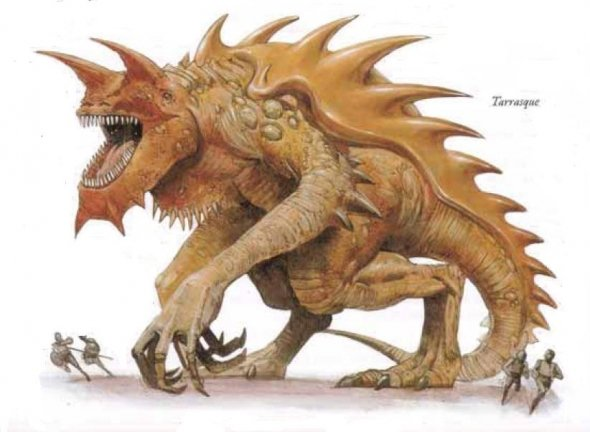
\includegraphics[height = 0.5\textheight, keepaspectratio = true]{tarrasque_1}
  \end{center}

\end{frame}

\begin{frame}
  \begin{center}
    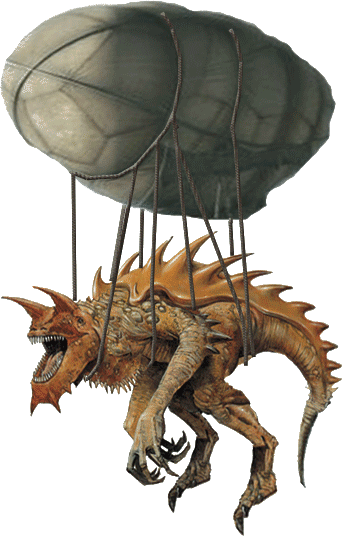
\includegraphics[height = \textheight, keepaspectratio = true]{tarrasque_2}
  \end{center}

\end{frame}

\begin{frame}
  \frametitle{Question 2}
  \Large{What does deathspell do?}

  While there is no ``deathspell'' there is a ``Finger of Death'' which is a close range spell that either kills the target or does large amounts of damage if the target is of great fortitude.

\end{frame}

\begin{frame}
  \frametitle{Question 3}
  \Large{Why is it a bad idea to steal a 20+ level mage's pouch?}

  Two words: spell selection.

  \small{
  \begin{quote}
  Imprison (9th level Abjuration): When you cast imprisonment and touch a creature, it is entombed in a state of suspended animation in a small sphere far beneath the surface of the earth. The subject remains there unless a freedom spell is cast at the locale where the imprisonment took place. Magical search by a crystal ball, a locate object spell, or some other similar divination does not reveal the fact that a creature is imprisoned, but discern location does. A wish or miracle spell will not free the recipient, but will reveal where it is entombed.
  \end{quote}
  }

\end{frame}

\section{Introduction}
%\subsection{Necessary History}
\begin{frame}
  \frametitle{Origin of Gygaxian Naturalism}
  \begin{columns}
    \begin{column}{0.5\textwidth}
      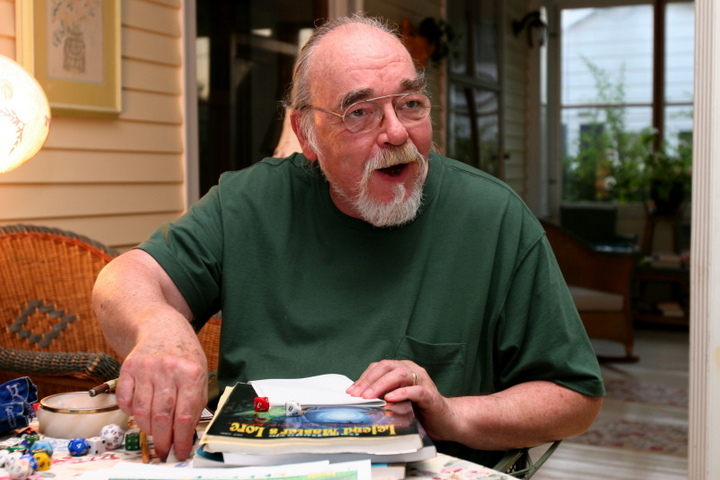
\includegraphics[width = \textwidth, keepaspectratio = true]{gygax}
    \end{column}
    \begin{column}{0.5\textwidth}
      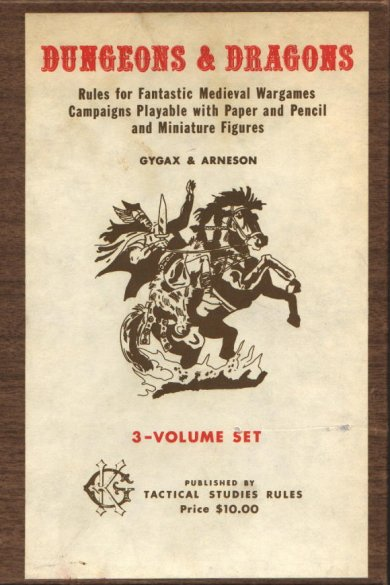
\includegraphics[width = \textwidth, keepaspectratio = true]{whitebox}
    \end{column}
  \end{columns}

\end{frame}

\begin{frame}
  \frametitle{Central Texts}
  \begin{center}
  \noindent
  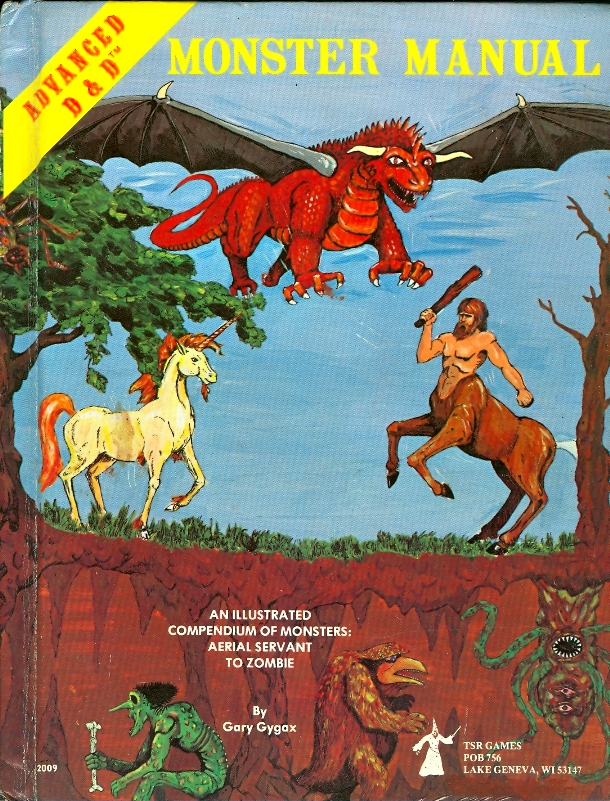
\includegraphics[height = 0.4\textheight, keepaspectratio = true]{mm1}\hspace{0.2\textwidth}%
  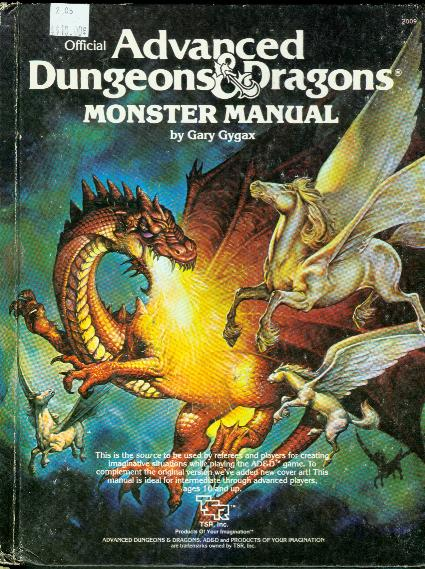
\includegraphics[height = 0.4\textheight, keepaspectratio = true]{mm2}\\[2em]
  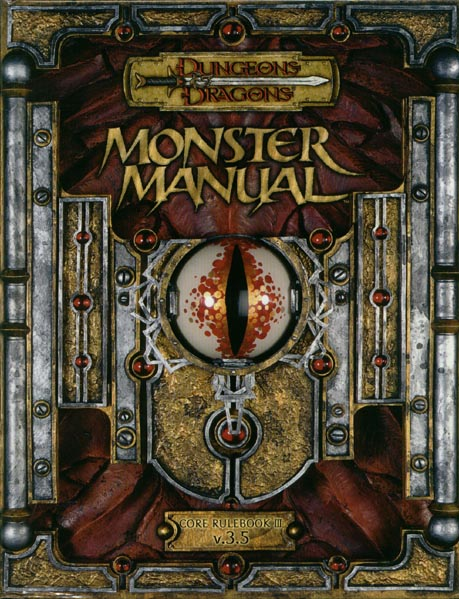
\includegraphics[height = 0.4\textheight, keepaspectratio = true]{mm35}\hspace{0.2\textwidth}%
  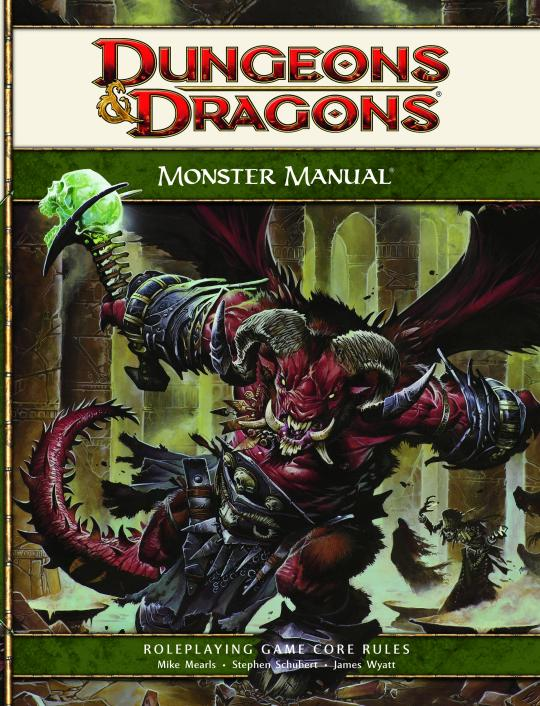
\includegraphics[height = 0.4\textheight, keepaspectratio = true]{mm4}\par
  \end{center}
  
\end{frame}

\begin{frame}
  \frametitle{Other Important Works}
  \begin{center}
  \noindent
  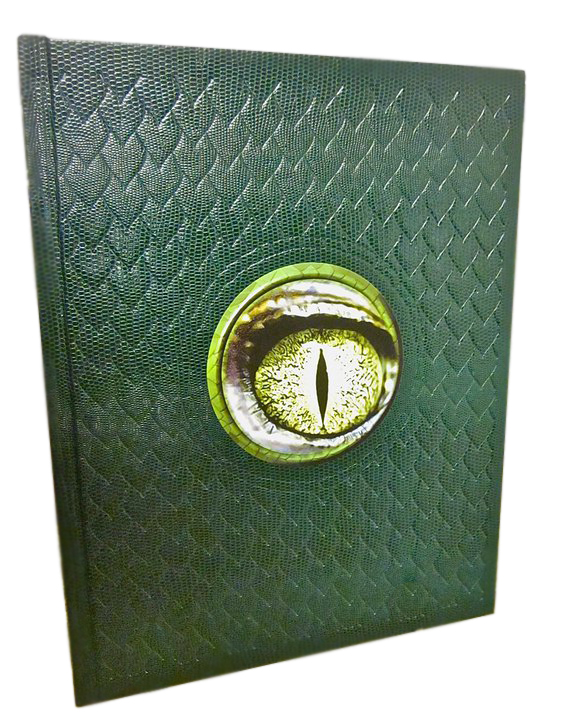
\includegraphics[height = 0.4\textheight, keepaspectratio = true]{hack}\hspace{0.2\textwidth}%
  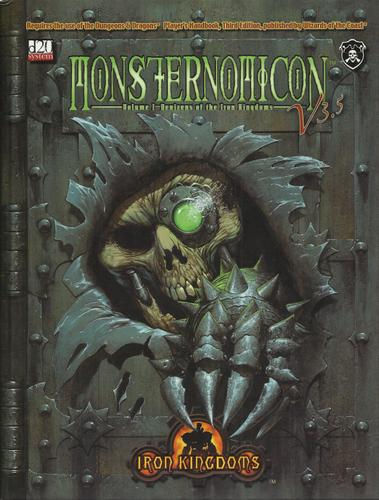
\includegraphics[height = 0.4\textheight, keepaspectratio = true]{nomicon}\\[2em]
  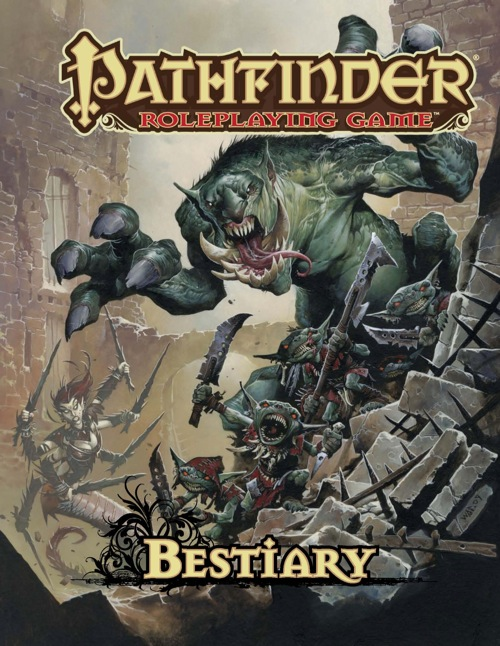
\includegraphics[height = 0.4\textheight, keepaspectratio = true]{path}\hspace{0.2\textwidth}%
  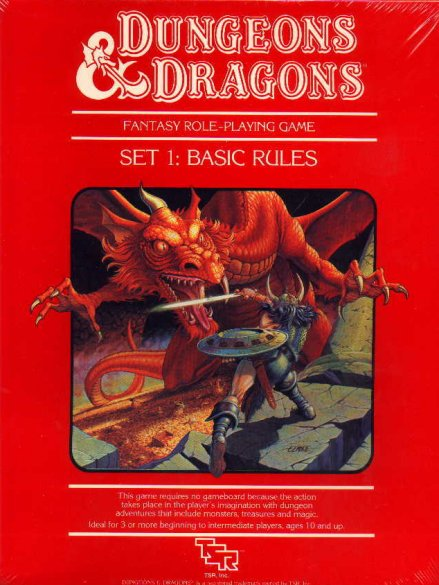
\includegraphics[height = 0.4\textheight, keepaspectratio = true]{redbox}\par
  \end{center}

\end{frame}

\begin{frame}
  \frametitle{Consistent Questions}
  \Large{
  \begin{itemize}
    \item How many species/monsters are there?
    \item Are many of the named species actually just subspecies?
    \item How much of diversity can be explained arcane forces?
    \item What is the species concept when magic can cause almost any two species to mate?
  \end{itemize}
  }

\end{frame}


\section{Goblinoid Phylogeny}
\begin{frame}
  \frametitle{How many goblinoids are there?}
  
  \begin{columns}
    \begin{column}{0.5\textwidth}
      \begin{itemize}
        \item Goblins
        \item Hobgoblins
        \item Bugbears
        \item Blues
        \\~\\
        \item Related taxa
        \begin{itemize}
          \item Orcs
          \item Ogres
          \item Ettins
          \item other monstrous humanoids
        \end{itemize}
      \end{itemize}
    \end{column}

    \begin{column}{0.5\textwidth}
      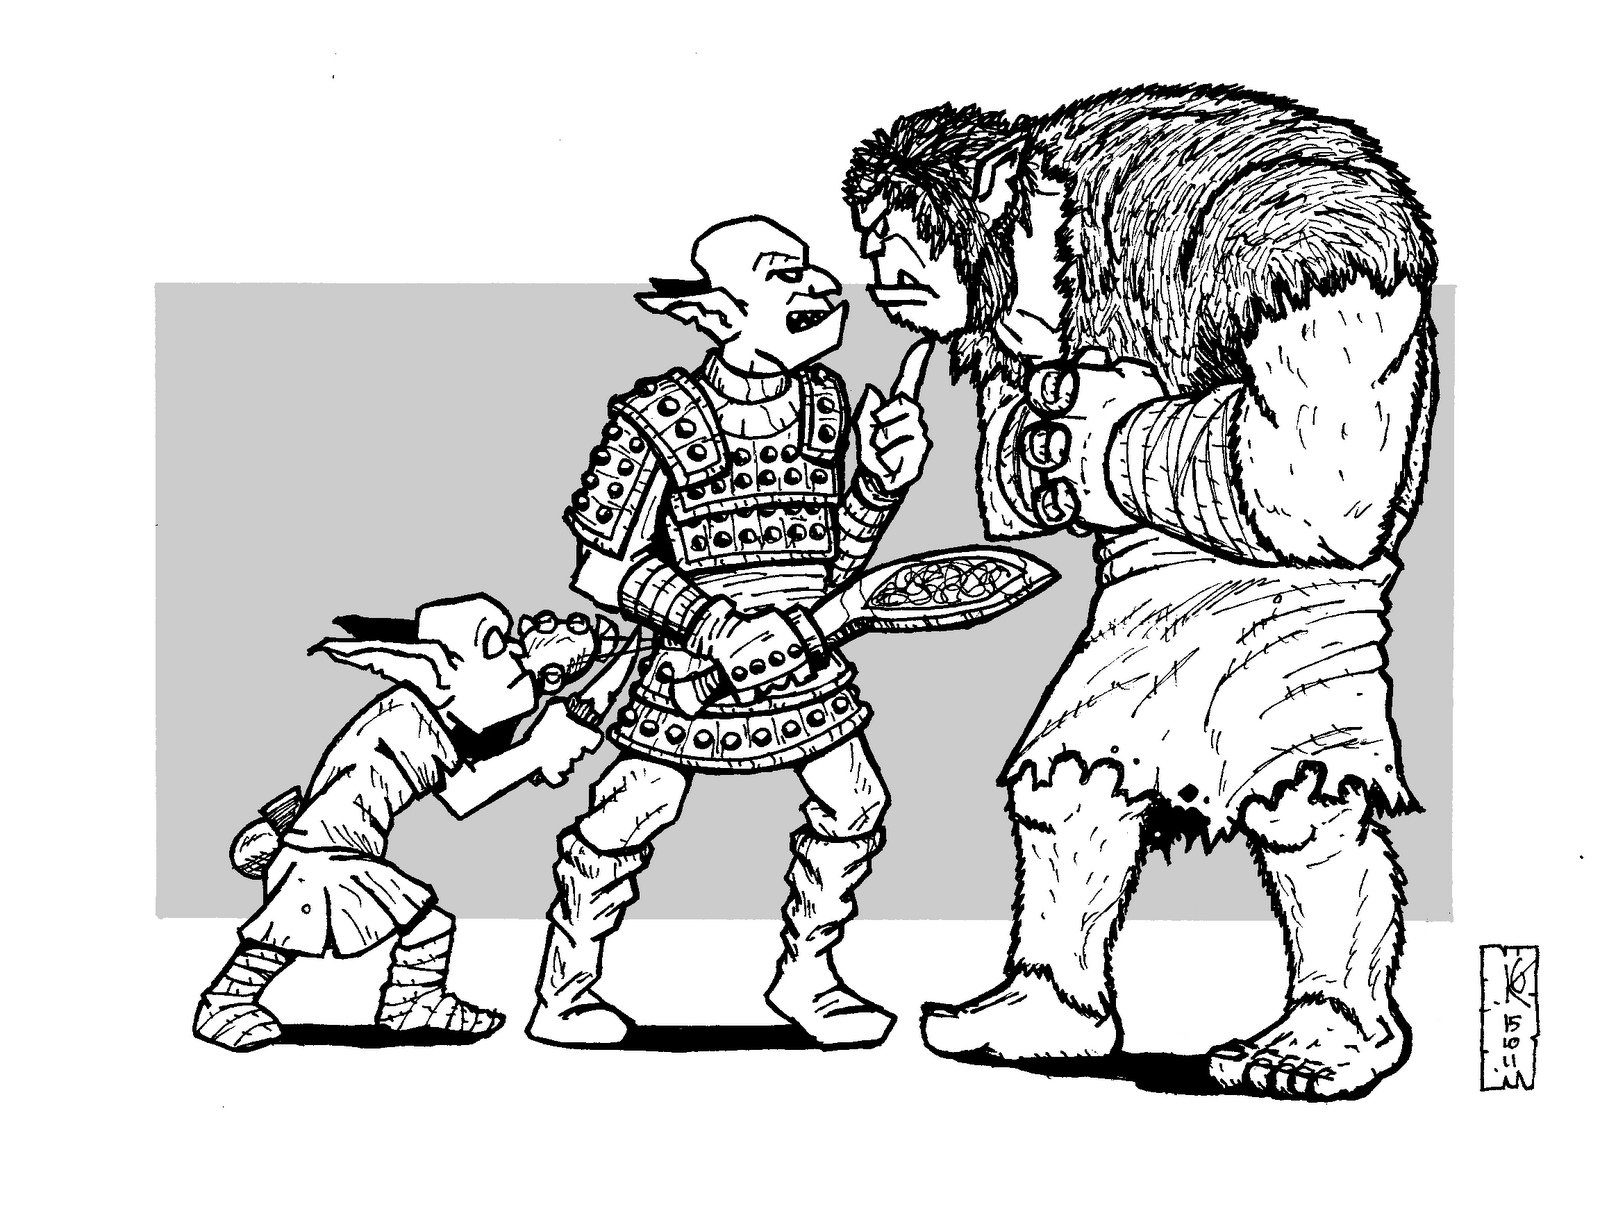
\includegraphics[width = \textwidth, keepaspectratio = true]{goblinoids}
    \end{column}

  \end{columns}

\end{frame}

\begin{frame}
  \frametitle{Materials and Methods}

  \begin{columns}
    \begin{column}{0.5\textwidth}
      \begin{itemize}
        \item Arcane, divine, morphological, behavioral characters
        \item Bayesian divination methods
        \item 20 prayer group of High Powered Clergy (HPC) operating through the Greyhawk Cathedral of Pelor
        \item Ritual took 8 hours.
      \end{itemize}
% Bayesian divination on the 
% HPC joke: H.. P.. Clergy
% operated by the Greyhawk Cathedral of Pelor
    \end{column}

    \begin{column}{0.5\textwidth}
      \begin{center}
        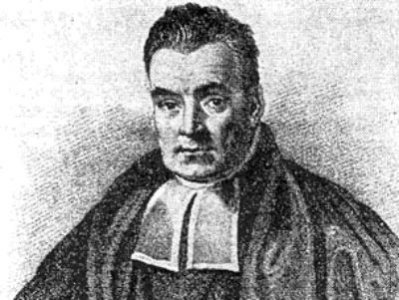
\includegraphics[width = 0.5\textwidth, keepaspectratio = true]{bayes}
        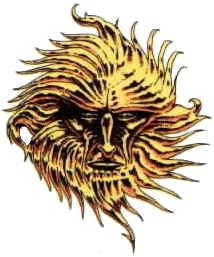
\includegraphics[width = 0.5\textwidth, keepaspectratio = true]{pelor}
      \end{center}

    \end{column}

  \end{columns}

\end{frame}

\begin{frame}
  \frametitle{Phylogeny}
\begin{knitrout}\scriptsize
\definecolor{shadecolor}{rgb}{1, 1, 1}\color{fgcolor}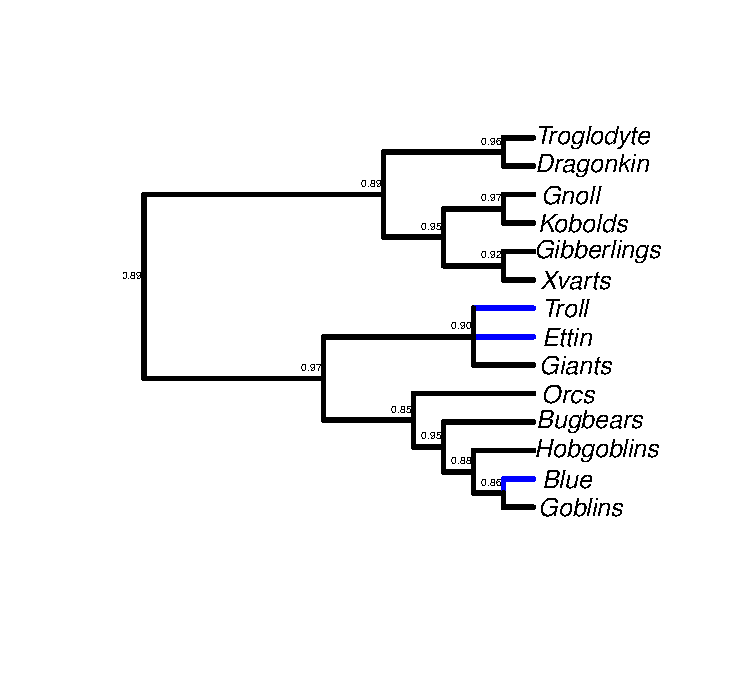
\includegraphics[width=\maxwidth]{figure/gob-phy} 
\end{knitrout}

\end{frame}


\section{Adaptation in Elves}
\begin{frame}
  \frametitle{History of our Knowledge}
  \begin{center}
    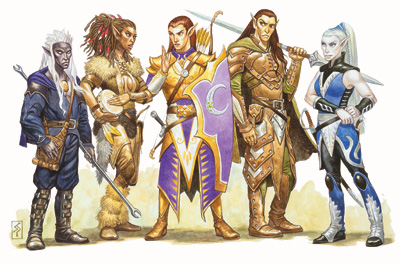
\includegraphics[height = 0.5\textheight, keepaspectratio = true]{elf_1}
  \end{center}

  At least 5 species/races of elves known from the most recent survey.

\end{frame}

\begin{frame}
  \frametitle{Adaptive or Cultural?}
  \begin{center}
    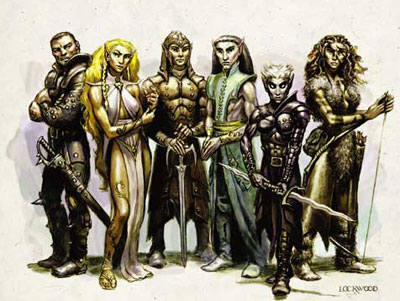
\includegraphics[height = 0.5\textheight, keepaspectratio = true]{elf_2}
  \end{center}

  All are adapted to very different environments, but physiologically and culturally.

\end{frame}

\begin{frame}
  \frametitle{Magic!!!}
  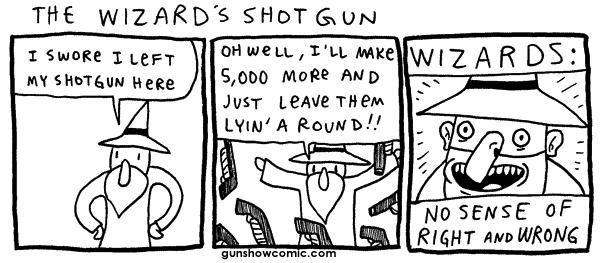
\includegraphics[width = \textwidth, keepaspectratio = true]{wizard_comic}

\end{frame}

\begin{frame}
  \frametitle{How else do explain\dots}
  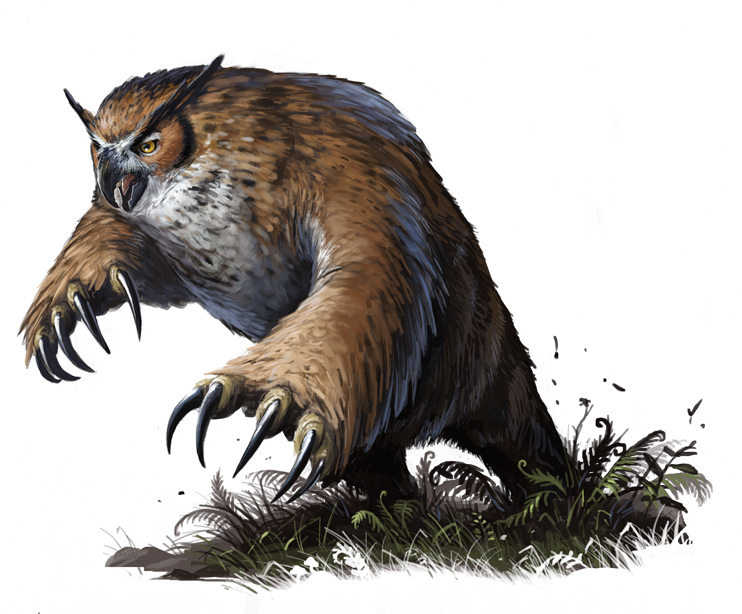
\includegraphics[width = \textwidth, keepaspectratio = true]{owlbear_1}

\end{frame}


\section{Species concepts with Dragons}
\begin{frame}
  \frametitle{}
  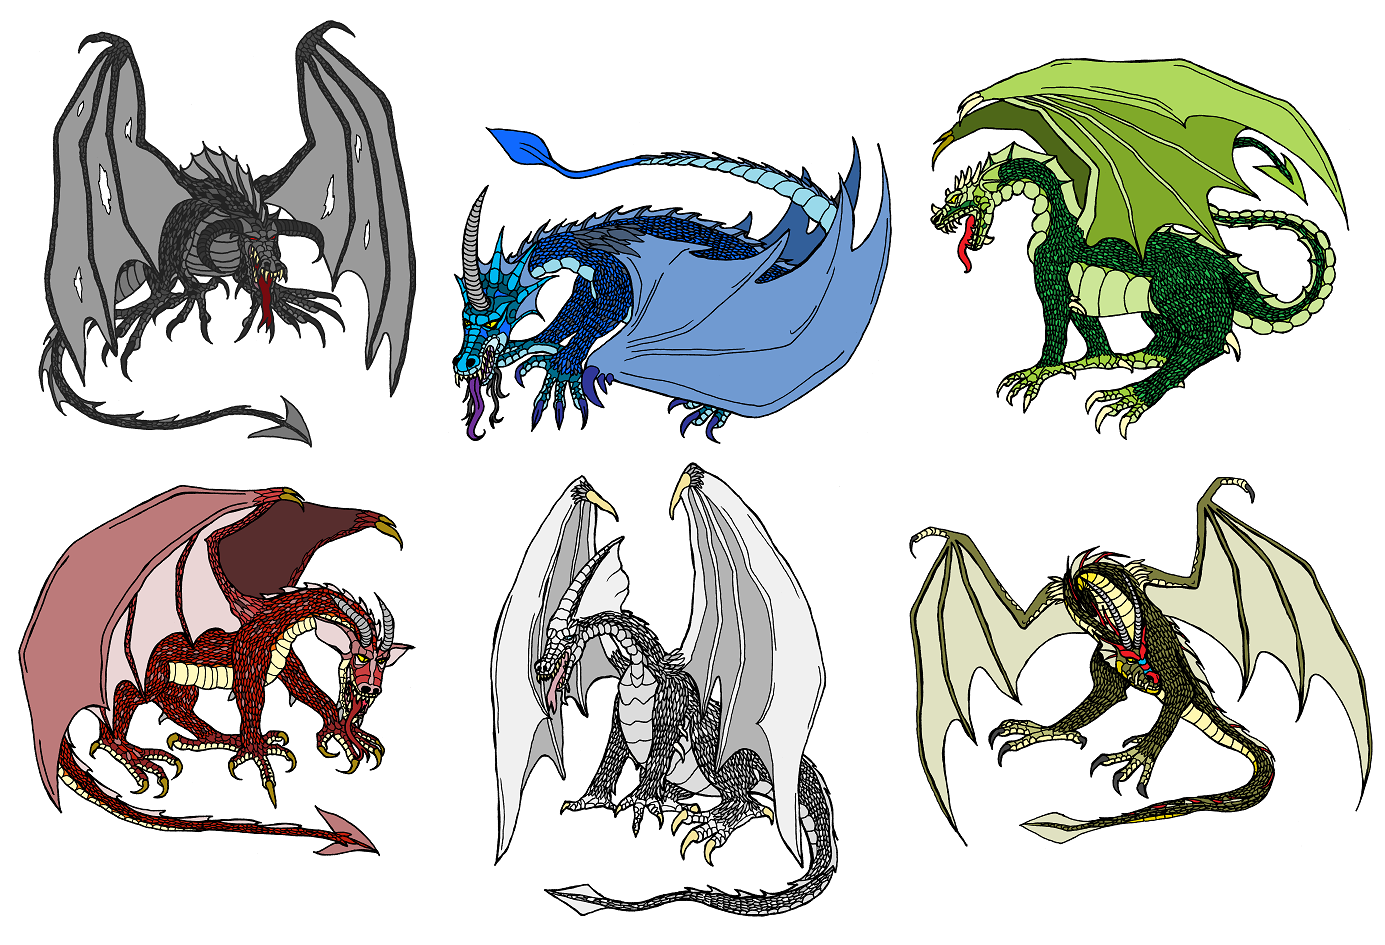
\includegraphics[width = \textwidth, keepaspectratio = true]{chromatic_1}

\end{frame}

\begin{frame}
  \frametitle{Violation of Biological Species concept}

  \begin{quote}
    The half-dragon template \dots can be applied to any corporeal creature. This demonstrates that dragons aren't selective regarding species. They're promiscuous.
  \end{quote}

  Dragons can successfully mate with all creatures from there plane. Including other dragons!

  Polymorph spells and magic in general prevent premating barriers. Pairings form viable offspring which are phenotypically heterotypic. Aspects of these phenotypes persist for generations, manifesting as ``mutations'' or innate magical talent.

\end{frame}

\begin{frame}
  \frametitle{Violation of Biological Species concept}

  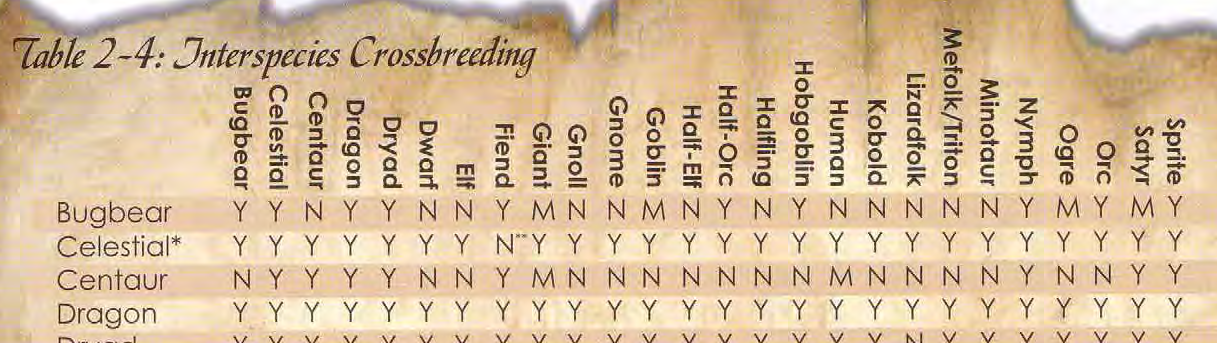
\includegraphics[width = \textwidth, keepaspectratio = true]{dragon_chart}

\end{frame}


\section{Dungeon Ecology}
\begin{frame}
  \frametitle{Dungeons verus all other biomes}

  Dungeons are continually reported as arcane biodiversity hotspots.

  These claims are frequently from amateur arcane biologists (adventurers) who are widely believed to be unreliable sources.

  Here, we compared multiple sites from 8 non-dungeon biomes and 6 different dungeon depths. Presented here for simplicities sake are only comparisons of entropy (Chao-Shen corrected).

  \footnotesize{Also, I'm lazy so don't blame me for using ``magic numbers.''}
% need to code so much to get this to work.
\end{frame}

\begin{frame}
  \frametitle{Results}
\begin{knitrout}\scriptsize
\definecolor{shadecolor}{rgb}{1, 1, 1}\color{fgcolor}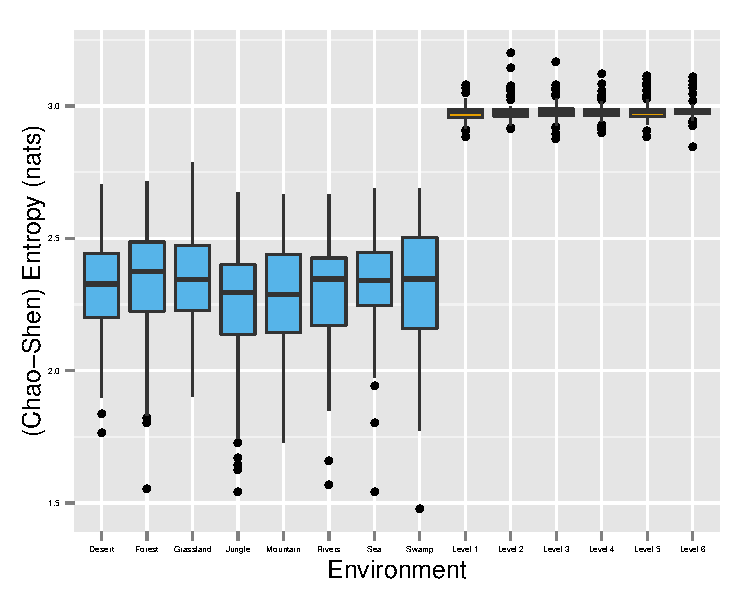
\includegraphics[width=\maxwidth]{figure/dungeon-eco} 
\end{knitrout}


\end{frame}


\section{Conclusions}

\begin{frame}
  \frametitle{Parting words}
  
  The world is a very scary place, full of monsters which want to kill and eat you. And maybe not in that order.

  Our understanding of these beings is distorted via the arcane energies that we ourselves use to better understand them.

  There will always be more creatures to find, though they might not be new ``species.''

  And sometimes\dots

\end{frame}

\begin{frame}
  \frametitle{\dots it is all just the will of the dice!}
  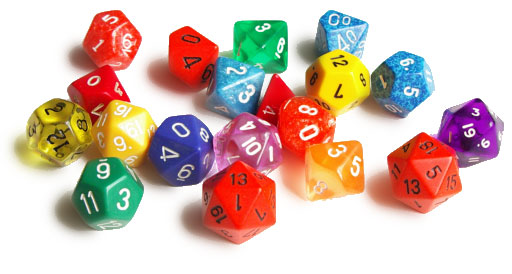
\includegraphics[width = \textwidth, keepaspectratio = true]{dice1}

\end{frame}


\begin{frame}
  \frametitle{Acknowledgements}

  \begin{columns}
    \begin{column}{0.5\textwidth}
      \begin{itemize}
        \item All my players though out the years
          \begin{itemize}
            \item The Crew of the Talking Pussy
            \item The Fancy Boots Brigade of Ruins
            \item New Corden Adventurers (temporary name)
            \item and all those without names
          \end{itemize}
        \item Rory Morrison to introducing me to role-playing games in the first place.
        \item \footnotesize{source available on GitHub}
      \end{itemize}

    \end{column}

    \begin{column}{0.5\textwidth}
      
\includegraphics[width = \textwidth, keepaspectratio = true]{unseen}

    \end{column}

  \end{columns}

\end{frame}


\end{document}
